%=============================================================================
\section{Introduction}
\label{sec:intro}
%=============================================================================

Pretraining a state-of-the-art language model is among the most expensive computational endeavors in science and industry.
A single frontier run consumes \$100--500M in compute, occupies thousands of GPUs for months, and processes trillions of tokens~\citep{deepseekv3, llama4, olmo2}.
Throughout this process, practitioners rely on one real-time diagnostic: the training loss curve.
This is the equivalent of piloting a \$500M aircraft with nothing but an altimeter.

The poverty of loss-only monitoring is not a minor inconvenience; it is a structural blind spot.
Loss can \emph{decrease} while model structure \emph{degrades}, because memorization reduces loss without improving generalization~\citep{overtraining_fragile2025}.
Loss is \emph{scale-dependent}: a value of 2.0 means different things for 1B and 7B models, making cross-model comparison impossible~\citep{hoffmann2022}.
The decision of \emph{when to decay the learning rate} is made by fixed schedules~\citep{wsd_schedule, li_schedules2026}, not by any signal from the model itself.
And there is no \emph{early warning} for training instability: loss spikes are detected only after the damage is done~\citep{deepseekv3, spectral_alignment2025}.

Results from Random Matrix Theory~\citep{martin_mahoney_jmlr2021, pennington2017, marchenko_pastur1967} and statistical physics~\citep{sadrtdinov2025, liu_tegmark2025, liu_ziyin_neurips2025} have shown that neural network weight matrices develop distinctive spectral signatures during training.
Well-trained layers exhibit \emph{heavy-tailed} eigenvalue distributions with power-law exponent $\alpha \in [2, 4]$, while untrained layers remain close to the random Marchenko-Pastur distribution ($\alpha > 6$)~\citep{martin_mahoney_jmlr2021}.
WeightWatcher~\citep{weightwatcher} demonstrated that $\alpha$ correlates with model quality across architectures, but only as a post-hoc diagnostic of fully-trained models.
How $\alpha$ \emph{evolves} during training, and whether spectral dynamics can serve as a real-time monitoring signal, remain open questions.

Our central observation is that spectral monitoring is not merely \emph{analogous} to statistical mechanics: it \emph{is} statistical mechanics.
The stable rank $\mathrm{SR} = \|W\|_F^2 / \sigma_1^2$ equals $\exp(H_{\text{R\'{e}nyi-2}})$, the exponential of the R\'{e}nyi-2 entropy of the normalized singular-value distribution~\citep{high_entropy_npj2026}.
When SR/$d$ converges to a universal constant, SGD is compressing the R\'{e}nyi-2 entropy of every weight matrix by approximately 2 nats, regardless of scale or architecture.
This is not analogy; it is a mathematical identity that grounds our framework in information-theoretic thermodynamics~\citep{wilson_compression_icml2025}.

In this work, we bridge the gap between static spectral analysis and real-time training guidance by tracking spectral properties across 13 language models, four architecture families, and nearly three orders of magnitude in scale (70M--65B) throughout training.
We establish four results:

\begin{enumerate}[leftmargin=*,itemsep=1pt,topsep=2pt]
    \item \textbf{A universal compression law} (\S\ref{sec:universal}). SR/$d$ converges to a value determined by hidden dimension $d$ alone, following $\mathrm{SR}/d \approx 0.040 + 0.61/\sqrt{d}$. Two models with identical $d = 5120$ but different depths (13B vs.\ 32B) achieve \emph{identical} SR/$d = 0.043$, confirming this is a layer-level property.

    \item \textbf{SR/$d$ as a quality predictor} (\S\ref{sec:predictor}). SR/$d$ achieves Spearman $r = -0.92$ with downstream benchmark performance across 102 checkpoint--benchmark pairs from 6 model scales, predicting quality from weights alone.

    \item \textbf{$\alpha$ reversal as early warning} (\S\ref{sec:reversal}). When $\alpha$ begins \emph{increasing} ($d\alpha/dt > 0$), spectral structure is degrading. This signal, invisible to loss, is \emph{model-size-dependent}: OLMo-2-13B shows $\Delta\alpha = +2.71$ despite $D/N = 365$, far above the threshold for smaller models, revealing that bigger models are more fragile.

    \item \textbf{An $\alpha$-guided adaptive schedule} (\S\ref{sec:schedule}). On FineWeb-Edu (10B tokens), an $\alpha$-guided schedule identifies the optimal decay point automatically (83\% of training), matching hand-tuned WSD ($\Delta\text{loss} < 0.004$) while outperforming cosine by $+1.95\%$ in downstream benchmarks.
\end{enumerate}

We additionally identify a \textbf{sharp structural phase transition at $N \approx 1.7$B parameters} (\S\ref{sec:scaling}): models below this threshold achieve heavy-tail structure ($\alpha < 3$) easily, while models above it remain structurally immature ($\alpha > 5$) even with hundreds of tokens per parameter. This ``Structural Chinchilla'' finding explains why over-training works for small models~\citep{gadre2024, muennighoff2023} and why frontier models remain spectrally immature despite massive compute~\citep{kaplan2020}. Per-layer heatmap analysis confirms that 96\% of structural ordering occurs in the first 4\% of training, after which the spectral state is largely frozen. We validate these findings on K2-65B, whose spectral metrics independently reveal its known benchmark underperformance (\S\ref{sec:audit}).

These results establish spectral monitoring as a practical complement to loss curves, grounded in the information-theoretic thermodynamics of SGD.
We release measurement code and monitoring dashboards for integration into existing training pipelines.

\begin{figure}[t]
    \centering
    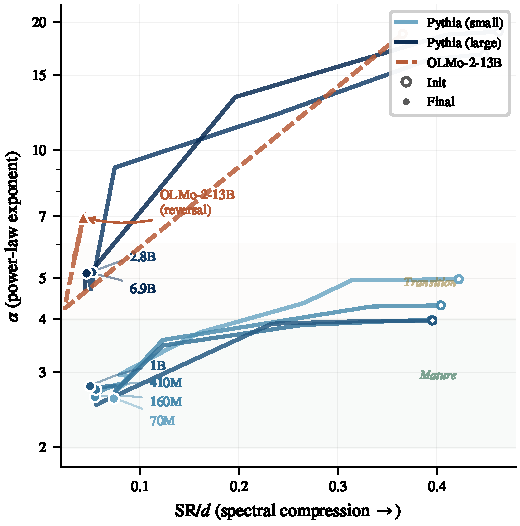
\includegraphics[width=0.85\columnwidth]{figures_v2/fig01_phase_portrait.pdf}
    \caption{\textbf{Spectral phase portrait.} Each model traces a trajectory through (SR/$d$, $\alpha$) space during training (right=init, left=final). Well-trained small models (70M--1B) converge to the lower-left ``mature'' region ($\alpha < 4$, SR/$d < 0.08$). Under-trained large models (2.8B, 6.9B) stall in the ``transition'' zone. OLMo-2-13B reverses direction after reaching its $\alpha$ minimum, moving \emph{away} from maturity. All models share the same compression axis (SR/$d$ converges universally) but diverge on the structural quality axis ($\alpha$).}
    \label{fig:phase_portrait}
\end{figure}
